%% Supplementary material for the IJCAS submission. Tables are generated by
%% paper/scripts/make_tables_v2.py; figures by paper/scripts/make_figures_v2.py.
\documentclass[10pt,a4paper]{article}
\usepackage[margin=20mm]{geometry}
\usepackage{mathptmx}
\usepackage{amsmath,amssymb}
\usepackage{graphicx,booktabs,url}
\usepackage[labelfont=bf]{caption}
\renewcommand{\thetable}{S\arabic{table}}
\renewcommand{\thefigure}{S\arabic{figure}}
\newcommand{\VfrozenKLexp}{-9}
\newcommand{\VextMeanLo}{0.79}
\newcommand{\VextMeanHi}{1.24}
\newcommand{\VextMax}{6.53}
\newcommand{\VfixL}{0.25}
\newcommand{\VfixG}{0.90}
\newcommand{\VfixLm}{0.25}
\newcommand{\VfixGm}{1.00}
\newcommand{\VadA}{0.10}
\newcommand{\VadB}{0.00}
\newcommand{\VrlppLmin}{0.20}
\newcommand{\VrlppLmax}{1.20}
\newcommand{\VrlppGmin}{0.84}
\newcommand{\VrlppGmax}{1.22}
\newcommand{\VrlppGstd}{0.11}
\newcommand{\VrLk}{-0.50}
\newcommand{\VrGk}{0.48}
\newcommand{\VrmseExpert}{1.07}
\newcommand{\VrmseDagger}{1.07}
\newcommand{\VrmseDP}{3.31}
\newcommand{\VrmsePPO}{7.40}
\newcommand{\VrmseFix}{0.90}
\newcommand{\VrmseAd}{0.63}
\newcommand{\VrmseRL}{1.03}
\newcommand{\VrmsePubBead}{4.38}
\newcommand{\VrmsePubRL}{5.00}
\newcommand{\VrmseFixOrig}{3.89}
\newcommand{\VrmseFixM}{0.77}
\newcommand{\VrmseAdM}{0.54}
\newcommand{\VrmseRLM}{0.88}
\newcommand{\VtExpert}{42.45}
\newcommand{\VtFix}{18.24}
\newcommand{\VtDP}{40.82}
\newcommand{\VtPPO}{50.04}
\newcommand{\VcompPPO}{25}
\newcommand{\VgPPO}{78.90}
\newcommand{\VnEpisodes}{2940}
\newcommand{\VrewExpert}{715}
\newcommand{\VrewDagger}{714}
\newcommand{\VrewDP}{624}
\newcommand{\VrewPPO}{517}
\newcommand{\VdiagDagDetrew}{746}
\newcommand{\VdiagDagDetrmse}{0.87}
\newcommand{\VdiagDagDett}{48}
\newcommand{\VdiagDagStorew}{766}
\newcommand{\VdiagDagStormse}{2.84}
\newcommand{\VdiagDagStot}{60}
\newcommand{\VdiagDPDetrew}{604}
\newcommand{\VdiagDPDetrmse}{3.90}
\newcommand{\VdiagDPDett}{45}
\newcommand{\VdiagDPStorew}{632}
\newcommand{\VdiagDPStormse}{4.26}
\newcommand{\VdiagDPStot}{53}
\newcommand{\VklLo}{0.005}
\newcommand{\VklHi}{0.016}
\newcommand{\VevLo}{0.71}
\newcommand{\VevHi}{0.92}
\newcommand{\VnRefs}{493}
\newcommand{\VnInst}{21}
\newcommand{\VnSynthEval}{100}

\graphicspath{{../revised/figures/}}
\makeatletter\let\tabinput\@@input\makeatother
% The shared tables name the expert by its equation number; in the paper it is Eq. (3).
\makeatletter\@ifundefined{r@eq:expert}{\@namedef{r@eq:expert}{{3}{}}}{}\makeatother

\title{Supplementary Material for\\``Learned Direct Actuation versus Tuned and RL-Tuned Pure Pursuit:\\A Controlled Comparison for Path Tracking''}
\author{Dileep Banothu and N. Sanjay Varma}
\date{}

\begin{document}
\maketitle

This supplement contains material moved from the main paper for length: the data split and the image-to-reference front end (Figs.~S1--S2), the waypoint spacing of every circuit reference (Table~S1), the results on the synthetic test contours (Table~S2), the per-circuit results of the naive-protocol contrast (Table~S3), and further views of the test-circuit results (Figs.~S3--S5). All numbers are generated from the released result files.

\begin{figure}[h]
\centering
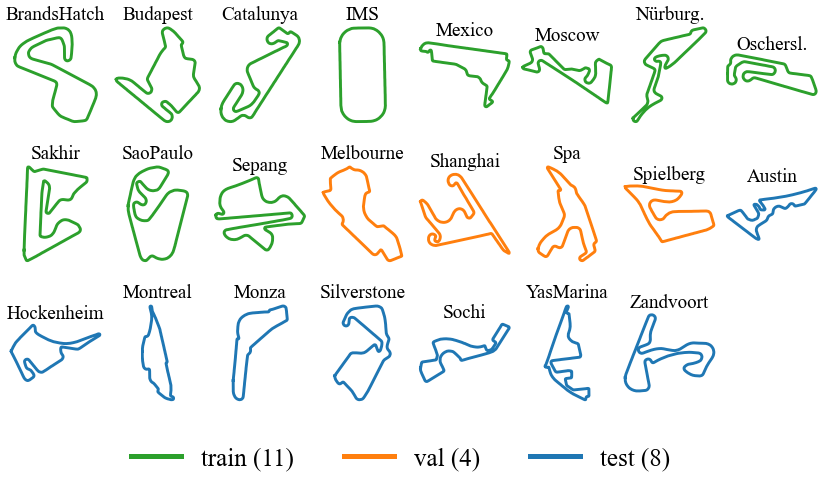
\includegraphics[width=0.7\textwidth]{fig2_split.png}
\caption{The 23 extracted F1TENTH references, with color indicating the split. Besides the three circuits that trained the naive-protocol bead (Yas Marina, Montreal, Hockenheim), five more form the test set; none of them is used to train, tune or select any controller.}
\end{figure}

\begin{figure}[h]
\centering
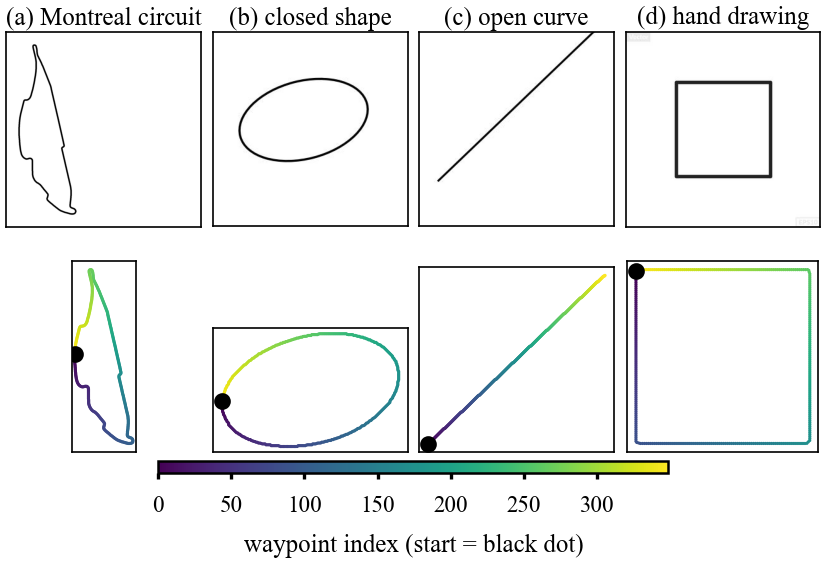
\includegraphics[width=0.7\textwidth]{fig8_inputs.png}
\caption{From image to reference path. Upper row: four inputs, namely one test circuit rendered as an image, one closed and one open synthetic test contour, and a hand drawing. Lower row: the ordered paths obtained from them, shaded by waypoint number, with waypoint 0 shown as a black dot.}
\end{figure}

\begin{table}[h]
\centering
\caption{Waypoint spacing of the extracted circuit references (median and range of the distance between consecutive waypoints). The expert of Eq.~(3) of the paper aims at the next waypoint, so its target lies \VspMin--\VspMax~cm ahead depending on the circuit; Pure Pursuit interpolates its lookahead point along the polyline.}
\small
\begin{tabular}{llccc}
\toprule
Circuit & Split & Waypoints & Median spacing [cm] & Range [cm]\\
\midrule
\tabinput ../revised/tables/tab_spacing.tex
\bottomrule
\end{tabular}
\par\vskip 2pt\parbox{\columnwidth}{\footnotesize$^\ddagger$Shortest segment is the last one, where the extracted loop stops short of its start and its final points hook back slightly; it is not a junction between pieces (no circuit reference has a break): Spielberg 5.6~cm, loop open by 8.2~cm, minimum of the other segments 15.7~cm; Austin 10.5~cm, loop open by 4.6~cm, minimum of the other segments 12.9~cm.
}
\end{table}

\begin{table}[h]
\centering
\caption{Accuracy on the synthetic test set of 100 contours; Geom@0.10 is given as average $\pm$ standard deviation over the contours, and the best entry of each set is bold. $^\ast$, $^\dagger$: naive protocol; $^\S$: Fixed PP law on the bead.}
\small
\begin{tabular}{lcccc}
\toprule
Set / Controller & Geom@0.10 [\%] & RMSE [cm] & Ordered [\%] & Time [s]\\
\midrule
\tabinput ../revised/tables/tab_shapes.tex
\bottomrule
\end{tabular}
\end{table}

\begin{table}[h]
\centering
\caption{Scores on the three circuits that trained the naive-protocol bead, as Geom@0.10 [\%] and RMSE [cm]; bold marks the best entry per column.}
\small
\begin{tabular}{lcccccc}
\toprule
& \multicolumn{2}{c}{Hockenheim} & \multicolumn{2}{c}{Montreal} & \multicolumn{2}{c}{Yas Marina}\\
Controller & G@0.10 & RMSE & G@0.10 & RMSE & G@0.10 & RMSE\\
\midrule
\tabinput ../revised/tables/tab_paper_circuits.tex
\bottomrule
\end{tabular}
\end{table}

\begin{figure}[h]
\centering
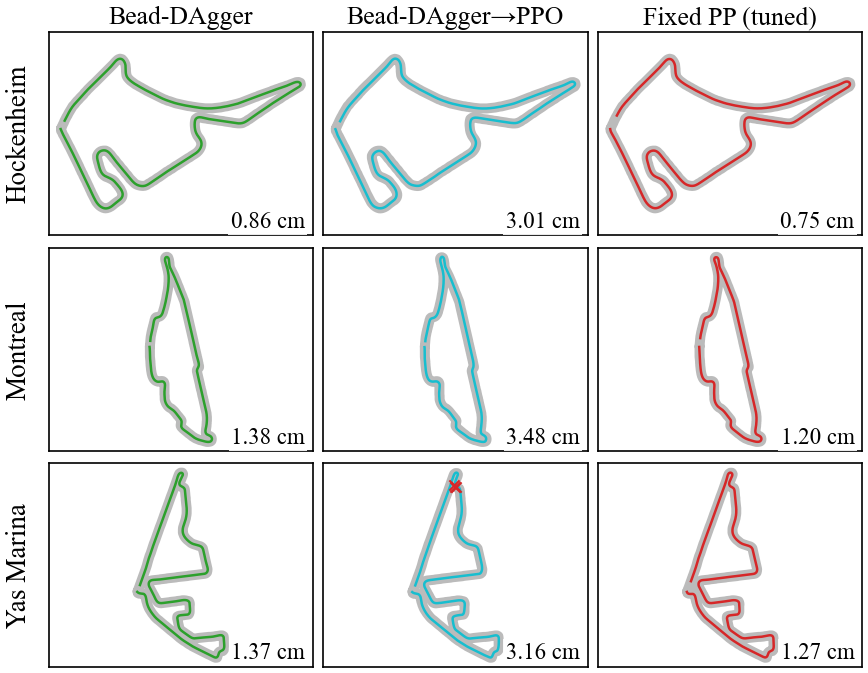
\includegraphics[width=0.6\textwidth]{fig9_traces.png}
\caption{Complete laps (first episode, seed 0) drawn over the grey reference on three unseen circuits. A red cross marks a reference point missed by more than 0.10~m (the start/finish join is ignored); the number in each panel is the RMSE of that lap.}
\end{figure}

\begin{figure}[h]
\centering
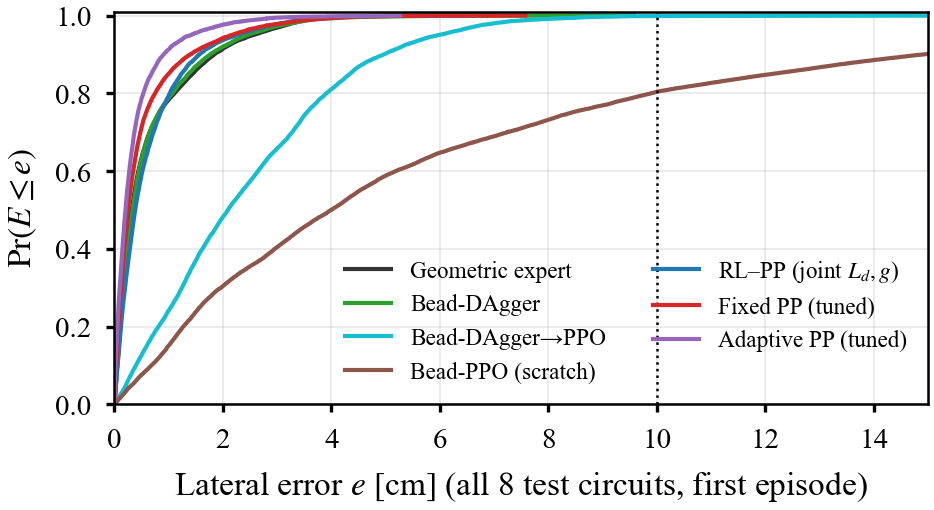
\includegraphics[width=0.6\textwidth]{fig11_cdf.png}
\caption{Fraction of trajectory samples whose distance to the extracted reference stays below a threshold, with all eight test circuits taken together (first episode; seed 0 for learned controllers). The dotted line is at 0.10~m.}
\end{figure}

\begin{figure}[h]
\centering
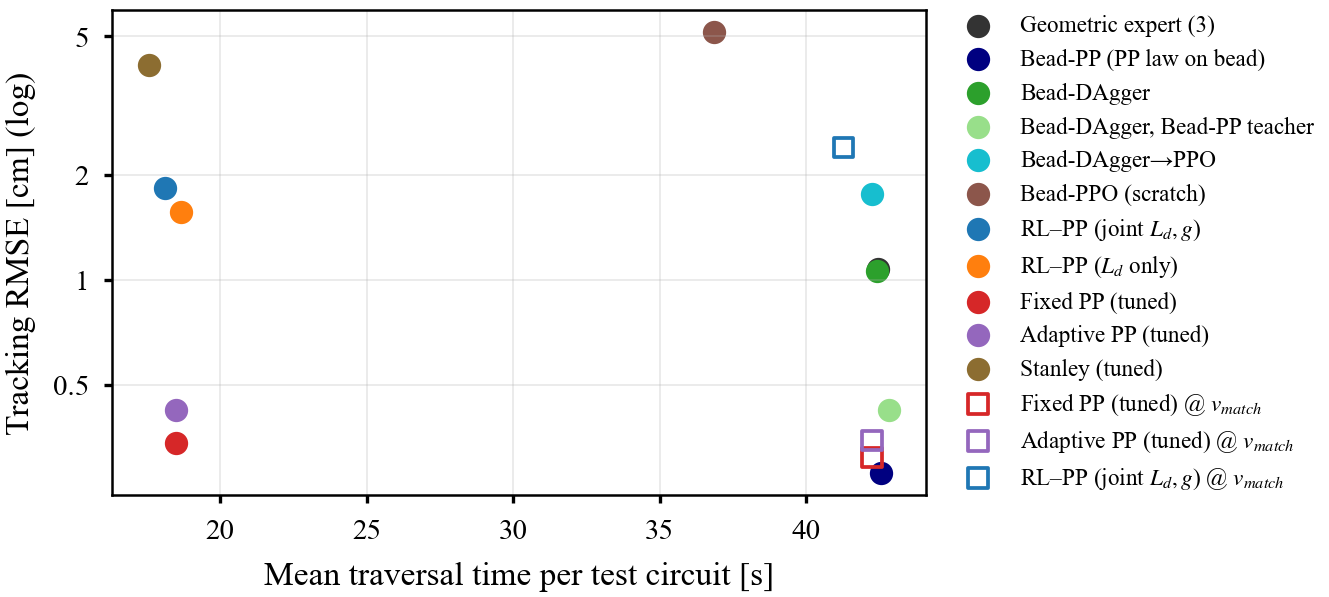
\includegraphics[width=0.6\textwidth]{fig4_pace.png}
\caption{Accuracy against lap time on the test circuits. Solid circles: every controller at its own speed (Track~A). Hollow squares: the car's PP-family controllers with their target speed limited to $v_{\mathrm{match}}$ (Track~B).}
\end{figure}

\begin{figure}[h]
\centering
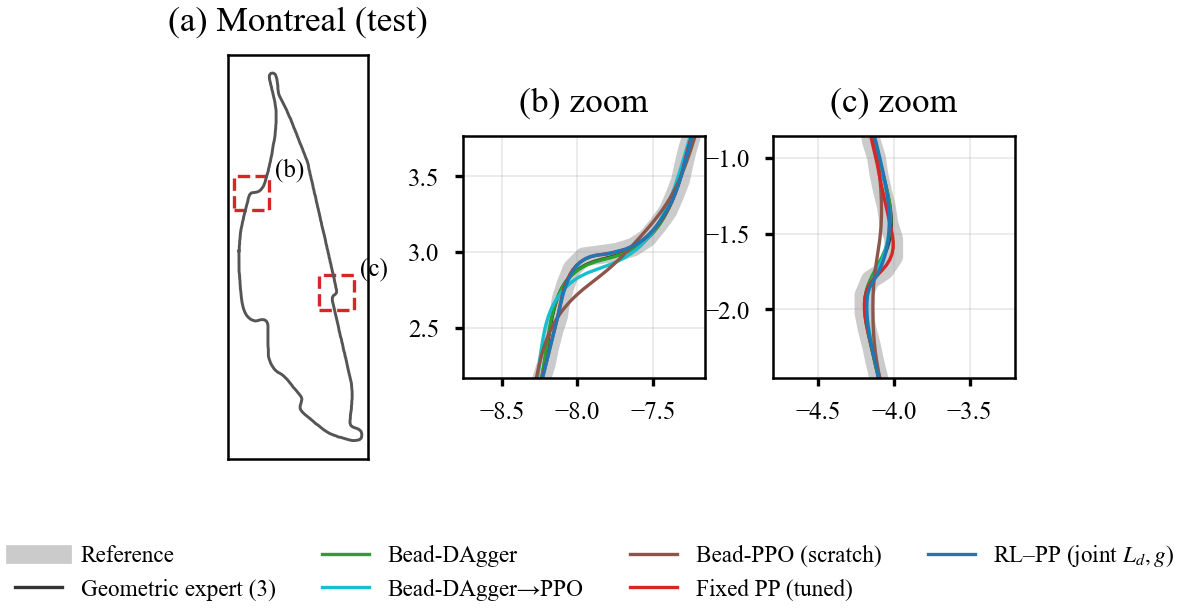
\includegraphics[width=0.6\textwidth]{fig6_zoom.png}
\vskip -0.5pc
\caption{Close-up of the controllers on the unseen Montreal circuit (first episode, seed 0). Both zoom windows are placed by the script at the two reference points where Bead-DAgger$\to$PPO strays furthest, leaving out the start/finish area.}\label{fig:zoom}
\vskip -1pc
\end{figure}

\end{document}
